
%(BEGIN_QUESTION)
% Copyright 2006, Tony R. Kuphaldt, released under the Creative Commons Attribution License (v 1.0)
% This means you may do almost anything with this work of mine, so long as you give me proper credit

A water pump recirculation valve has a full-open C$_{v}$ rating of 20.  If the pump outputs a flow of 700 GPM of water at a differential pressure (outlet pressure - inlet pressure) of 100 PSID, what will be the total water flow output by the system when the bypass valve is 100\% open?

$$\includegraphics[width=15.5cm]{i01374x01.eps}$$

\vskip 20pt \vbox{\hrule \hbox{\strut \vrule{} {\bf Suggestions for Socratic discussion} \vrule} \hrule}

\begin{itemize}
\item{} This control valve arrangement -- where the valve recirculates water flow from discharge to suction -- is far preferable to one where a valve simply blocks off the pump discharge.  Explain why recirculation is better than blockage as far as control valve placement is concerned.
\end{itemize}

\underbar{file i01374}
%(END_QUESTION)





%(BEGIN_ANSWER)

 
%(END_ANSWER)





%(BEGIN_NOTES)

$Q_{outlet}$ = 500 GPM

\vskip 10pt

Given a 100 PSI differential pressure drop across the valve, and a flow coefficient of 20, the valve will bypass 200 GPM of water.  If the pump's output is 700 GPM, and the valve bypasses 200 GPM of that flow, the final outlet flow from the system will be the difference between these two flow rates, or 500 GPM.

It should be noted that this method of flow control on a water pump is much preferable to locating the valve in-line with the pump discharge.  Water pumps may be damaged if their discharge is blocked, and this is what will happen when an in-line valve ever closes.  Bypass valves do not cause this same problem.

%INDEX% Final Control Elements, valve: sizing

%(END_NOTES)


